A \cuda{} thread is a lightweight thread (compared to a normal CPU thread).
As a kernel is executed in parallel by multiple threads, there must be a way to distinguish each thread from one another, so that they can perform different work.
Each thread is therefore given a \textit{thread index}, which can be accessed by each thread when executing a kernel.
It is syntactically done by accessing the struct \textit{threadIdx}, which contains the thread id in 3 dimension (x,y,z).
A simple example can be seen in \autoref{lst:threadIdx}.
\begin{lstlisting}[language=C,caption={Thread index example},label=lst:threadIdx]
__global__ void thread_idx_example(float* d_out, float* d_in){
	int idx = threadIdx.x;
	int idy = threadIdx.y;
	int idz = threadIdx.z; }
\end{lstlisting}


threads / block dim etc
thread id (in a block )etc

The thread hierarchy can be seen in \autoref{fig:grid-of-thread-blocks}, where the numbering is shown in "(x,y)".
\begin{figure}[ht]
	\centering
	\fbox{
		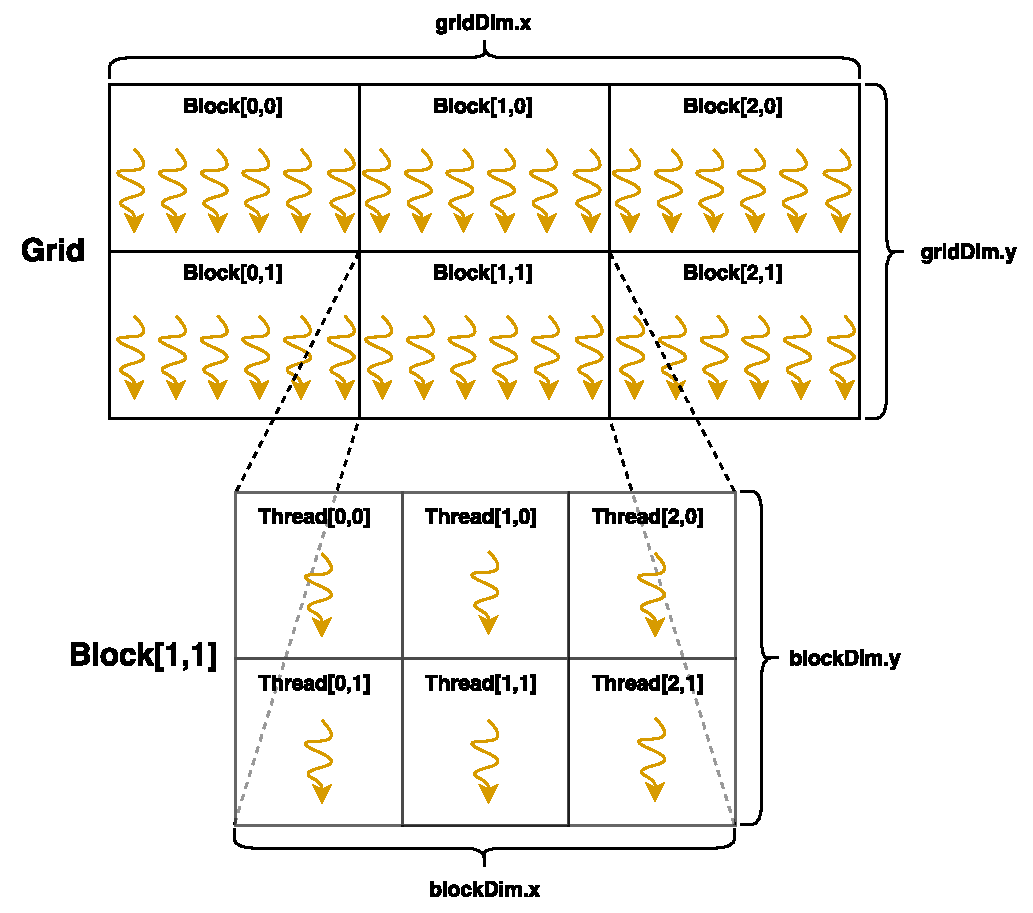
\includegraphics[width=0.6\textwidth]{figs/programming-model/grid-of-thread-blocks.pdf}
	}
	\caption{Grid of thread blocks}
	\label{fig:grid-of-thread-blocks}
\end{figure}